\documentclass[../main.tex]{subfiles}

\begin{document}
	\section{Les bases}
	On trouve trois grandes classes de polymère, les Thermoplastiques, les thermodurcis et les élastomères. 
	\begin{enumerate}
		\item Thermoplastiques
		\begin{itemize}
			\item Solides plus ou moins durs
			\item Amorphe ou semi-cristallin
			\item Plastique ou cassant
			\item Molécule linéaire ou branchées
			\item Liquide à température élevée
		\end{itemize}
		\item Elastomères
		\begin{itemize}
			\item Solides mous
			\item Grandes déformations réversibles
			\item Faible densité de réticulation
		\end{itemize}
		\item Thermodurcis
		\begin{itemize}
			\item Solide dur
			\item Amorphe
			\item Cassant
			\item Forte densité de réticulation
		\end{itemize}
	\end{enumerate}

	\section{Polymère usuels}
		\subsection{Les 5 grands thermoplastiques}
		On trouve 5 grand thermoplastiques qui sont bon marché et utilisé dans la vie courante
		\begin{enumerate}
			\item Polyéthylène haute densité (HDPE)
			\item Polyéthylène basse densité (LDPE)
			\item Poly chlorure de vinyle (PVC)
			\item Polystyrène (PS)
			\item Polypropylène isotactique (PP)
		\end{enumerate}
		\subsection{Thermoplastiques techniques}
		Les thermoplastiques techniques sont composé de structures souvent relativement complexes (comparé aux grand 5) et sont plus chères que ceux ci. Ils sont généralement plus performants que les 5 grands
		\begin{enumerate}
			\item Polycarbonate (PC)
			\item Polyexyméthylène (POM)
			\item Polyéthylène téréphtalate (PET)
			\item Polyamide (PA)
			\item Polytetrafluoroéthylène (PFTE)
			\item Poly ether ether cétone (PEEK)
		\end{enumerate}
		\subsection{Thermodurcis}
		Ce sont en général des résines à faible masse molaire et peu visquese, réticulées pendant la mise en oeuvre par apport de chaleur ou irradiation.
		\begin{enumerate}
			\item Epoxydes
			\item Polyester insaturé
			\item Phénolique
			\item Mélamines
			\item  Polyuréthanes (PUR)
		\end{enumerate}
		Les thermodurcis, contrairement aux thermoplastiques, ne sont pas recyclable. On les trouves dans des boitiers ou emballages, pour des isolations électriques ou thermiques. Ils sont également utilisé pour l'impression 3D. Enfin une dernière application se trouve dans les polymères bioactis, qui permettent de combiner les fonctions avec les caractéristiques spécifiques des polymères (souplesse et/ou transparence).
		\subsection{Elastomères}
		Les élastomères sont la famille des caoutchouc. En fait le caoutchouc est un elastomère naturel, alors qu'on dénomme en général élastomère par matériau synthétique. Ils permettent d'importantes élongations (jusqu'à $500-1000\%$) qui sont réversibles.
		Ils sont reliés par des liaisons covalentes croisées.
		\section{Structure de base}
		\subsection{Méthodes de synthèse}
		Il y a deux principaux types de synthèse. Les 5 grands sont généralement polymérisés par addition radicalaire (fig. \ref{additionradicalaire}) et les polymères techniques par polycondensation (fig. \ref{polycondensation}).
		
		\begin{figure}[h]
			\begin{center}		
			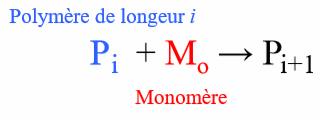
\includegraphics{AdditionRadicalaire.png}
			\caption{\label{additionradicalaire} Principe d'addition radicalaire utilisé par les 5 grands.}
			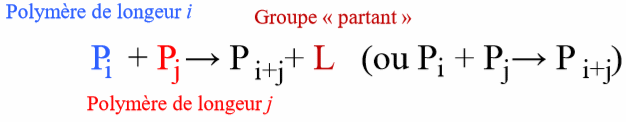
\includegraphics{PolyCondensation.png}
			\caption{\label{polycondensation} Principe de polycondensation utilisé par les techniques. Nous avons ici un produit des chaînes linéaires (X réagit sur Y) $X-X + Y-Y  \rightarrow X-XY-XY-XY...$} 
			\end{center}
		\end{figure}
		La polymérisation par addition est typiquement très rapide. La terminaison est due aux impuretés, aux recombinaison de radicaux libre ou aux dismutations. Les liaisons sont ouvertes grâce à l'amorçage (par un radical libre).
		
		La polycondensation pour le PET par exemple fonctionne avec deux fonctions capable de réagir l'une avec l'autre ($acide + alcool$ ou $aldehyde + amine$).
		
		Les polymères sont des mélanges. A cause des variations statistiques durant le procédé de polymérisation, les polymères même dans leur forme la plus pure, sont en fait des mélanges de mlécules de différente masse moléculaires. 
		Dans la pratique on se sert en général des différentes masses moyennes.
		
		La masse moyenne en nombre, $M_n$ est définie sur base du nombre $n_i$ des chaînes de masse $M_i$ présente dans le mélange. 
		\begin{equation}
			M_n = \frac{\sum_{i}n_iM_i}{\sum_{i}n_i} 
		\end{equation}
		
		La masse moyenne en poids, $M_w$, est calculée à partir des fractions en poids, $w_i$ des chaînes.
		\begin{equation}
			M_w = \frac{\sum_{i}w_iM_i}{\sum_{i}w_i} =  \frac{\sum_{i}n_iM_i^2}{\sum_{i}n_iM_i}
		\end{equation}
		Le rapport $I = \frac{M_w}{M_n}$ est toujours plus grand que l'unité. Il s'appelle polydispersité ou indice de polymolécularité. 
		
		\subsubsection{Importance de la polydispersité}
		En général, plus $M_n$ et $M_w$ sont élevés, plus on améliore les propriétés. Si $M_w$ est trop faible, on perd toutes les propriétés caraactéristique d'un polymère.
		Dans l'autre sens, si $M_w$ est trop élevé, la viscosité devient trop élevée pour permettre la mise en forme à l'état fondu. Une très grande polydispersité I peut palier ce problème jusqu'à un certain point.
		\subsection{Configuration}
		La Configuration est l'arrangement dans l'espace tridimensionnel des atomes ou groupes attachés à un atome central. Pour passer d'un isomère configurationnel a un autre, on est obligé de casser des liaisons covalentes. 
		\begin{figure}[h]
			\begin{center}
				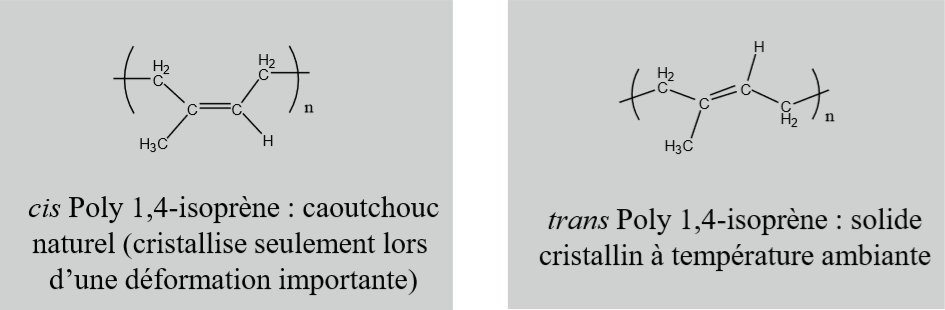
\includegraphics[width=18cm]{Conformation.png}
				\caption{\label{conformation}Par exemple le $Poly 1,4 isoprene$ qui en configuration \textit{cis} est un caoutchouc naturel et en configuration \textit{trans} est un solide cristsallin.}
			\end{center}
		\end{figure}
	
		\subsubsection{Tacticité}
		\begin{figure}[h]
			\begin{center}
				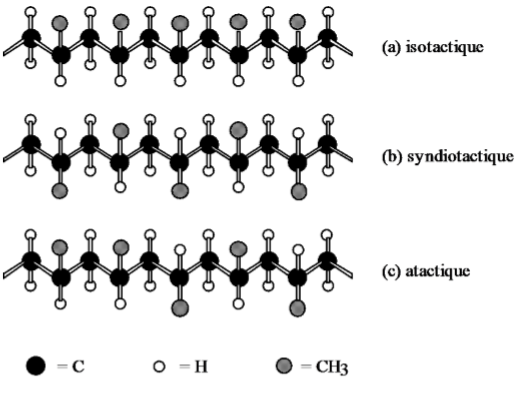
\includegraphics[width=18cm]{Tacticite.png}
				\caption{\label{tacticite}Cristallisation du PP qui lui donne des propriétés utiles pour la plupart de ses applications.}
			\end{center}
		\end{figure}
		En général, un cristal est un arrangement périodique régulier de chaînes alignées (fig. \ref{tacticite}). Si on a une configuration \textit{atactique}, les groupes $CH_3$ du polypropylène seront disposés aléatoirement de part et d'autre des chaînes, ce qui est incompatible avec un arrangement régulier. Le polypropylène atactique ne peut pas cristalliser et comme sa température de vitrification est assez faible, il se comporte comme un caoutchouc à température ambiante. 
		
		\subsection{Copolymère}
		L'intérêt des copolymère est de générer de nouveaux polymères avec de nouvelles propriétés. Par exemple dans le cas du PSAN, un copolymère statistique, on a un mélange intime de deux type de monomères. Le PS est un polymère bon marché mais cassan. Le PAN est un polymère performant mais difficile à transormer. En les combinant, on obtient une moyenne des propriétés de ces polymères. On essaie ainsi d'obtenir un bon compromis entre propriétés et mise en oeuvre.
		
		
\end{document}